\documentclass[conference]{IEEEtran}
\usepackage{cite}
\usepackage{amsmath,amssymb}
\usepackage{array}
\usepackage{booktabs}
\usepackage{url}
\usepackage{tikz}
\usetikzlibrary{positioning,arrows.meta}

\begin{document}

\title{Resource-Efficient Neural Architectures for Post-Disaster Damage Assessment and Rescue Guidance\\[1pt]
{\normalsize\itshape CSE499B/EEE499B/ETE499B -- Senior Design II, Section 15 --- Project Group 5 --- Review Report}}

\author{
\IEEEauthorblockN{Abdullah Al Noman}
\IEEEauthorblockA{ID: 2022095042}
\and
\IEEEauthorblockN{Tamanna Akter Mou}
\IEEEauthorblockA{ID: 2211951042}
\and
\IEEEauthorblockN{Aryan Sami}
\IEEEauthorblockA{ID: 2231407042}
\and
\IEEEauthorblockN{Ridita Afrin Riya}
\IEEEauthorblockA{ID: 2211622042}
\and
\IEEEauthorblockN{Abrar Mohammed Tanzim Alam}
\IEEEauthorblockA{ID: 2222864042}
}

\maketitle

\begin{abstract}
Disaster responders need building-level damage information, meaning where buildings collapsed and how many, within hours, offline and on modest hardware. In CSE499A we fine-tuned Qwen2.5-VL-7B on the DisasterM3 benchmark with QLoRA on one free T4 GPU and added a U-Net for counting. Two weaknesses remained: the vision-language model (VLM) lost 10.62 points on building counting, and the U-Net segmented destroyed buildings, 0.33\% of all pixels, at only 0.166 IoU. This review reports the first phase of CSE499B, a four-track segmentation ablation sprint over data balancing, decoder architecture, loss and backbone, and input resolution. A Focal Tversky loss gave the largest single gain (+0.056 mIoU); the best run reached 0.5296 mIoU and 0.279 Destroyed IoU, meeting the mIoU target but not the 0.30 Destroyed target. Because an audit found that the sprint's numbers were not comparable, we define one full-resolution evaluation protocol and a controlled champion-model plan (runs R1--R8 and E0), whose first runs reach 0.544 mIoU but only 0.284 Destroyed IoU. Finally, we outline four structural directions, before/after input, building-level grading with SAM~3, a tool-using VLM with offline reports, and edge-sized models, combined in one proposed offline architecture.
\end{abstract}

\begin{IEEEkeywords}
Disaster response, semantic segmentation, class imbalance, ablation study, Focal Tversky loss, vision-language models, QLoRA, knowledge distillation
\end{IEEEkeywords}

\section{Introduction}
After an earthquake, flood or explosion, satellite imagery arrives long before ground surveys can cover the affected area. Turning it into decisions, such as which blocks to search first or where teams can stage safely, requires knowing which buildings are damaged or destroyed and how many. Vision-language models (VLMs) describe disaster scenes fluently but estimate counts poorly, while segmentation networks localise damage pixel by pixel but struggle with rare classes.

In CSE499A we reproduced the DisasterM3 benchmark~\cite{disasterm3} by fine-tuning Qwen2.5-VL-7B~\cite{qwen25vl} with QLoRA~\cite{qlora} on a single 16\,GB T4. The model reached a six-task average of 31.39\% (base model 31.2\%; the paper's 4$\times$H100 model 40.4\%). It gained 11.69 points on bearing-body recognition but lost 10.62 points on building damage counting (BDC), because a 512-token image cap hides small structures. We therefore routed counting questions to a U-Net~\cite{unet}, which reached 0.4619 mIoU but only 0.1658 IoU on destroyed buildings. Supporting modules included DisasTeller, a CrewAI~\cite{crewai} multi-agent report generator running on the Gemini API; a DisasterVQA~\cite{disastervqa} evaluation (91.18\% binary accuracy, tying GPT-4.1-mini); and a VRT~\cite{vrt} super-resolution study.

CSE499B first strengthens the weakest link, the segmentation stage, then turns the modules into one offline system. This review contributes (i) a four-track, one-variable-at-a-time ablation sprint; (ii) an audit of its results and a single evaluation protocol; (iii) a controlled champion-model plan with its first results; and (iv) four future directions combined in a proposed offline architecture.

\subsection{Problem Statement}
Given a post-disaster optical satellite image and, where available, its pre-disaster counterpart, produce (i) a four-class building-damage map (background, intact, damaged, destroyed), (ii) per-class building counts derived from that map, and (iii) structured rescue guidance, such that: (a) destroyed buildings, only 0.33\% of pixels, are segmented with IoU above 0.30 at mIoU above 0.52 on full-resolution validation images; (b) counting answers come from the map rather than from VLM estimation, beating the untuned VLM's 34.2\% BDC accuracy; and (c) the pipeline runs with no proprietary API on free 16\,GB GPUs, with a distilled variant targeting about 6\,GB.

\subsection{Scope and Assumptions}
\textit{In scope:} optical DisasterM3 imagery, including the pre-disaster image paired with each post-disaster image; four-class, building-level damage assessment; the CSE499A fine-tuned VLM and modules; free-tier compute (Kaggle T4). \textit{Out of scope:} SAR imagery, real-time video, physical survivor detection, and any use as an authoritative directive without human review.

\section{Background}
DisasterM3~\cite{disasterm3} has about 123k instruction pairs over nine tasks, 92,968 of them in its training release; its referring-expression segmentation task supplies the intact, damaged and destroyed building masks that we merge into four classes. xBD~\cite{xbd} established pixel-level damage assessment and is our candidate external dataset. Against class imbalance, the Focal Tversky loss~\cite{focaltversky} weights false negatives above false positives and focuses on hard pixels, the Lov\'asz-Softmax loss~\cite{lovasz} is a convex surrogate of IoU, and copy-paste augmentation~\cite{copypaste} multiplies rare instances. We compare the U-Net~\cite{unet} with the UNet++~\cite{unetpp} and DeepLabV3+~\cite{deeplab} decoders. For deployment, sequence-level knowledge distillation~\cite{seqkd} trains a small student on a teacher's outputs, and SAM~3~\cite{sam3} segments every instance of a concept named by a short text prompt.

\section{Objectives and Key Results}
\textbf{O1. Strengthen the spatial stage.} KR1: a champion U-Net passes the Phase Gate on full-resolution validation images, with mIoU $>0.52$ and Destroyed IoU $>0.30$.

\textbf{O2. Ground the VLM spatially.} KR2: hybrid counting (champion U-Net plus a higher-resolution VLM) beats the base model's 34.2\% BDC accuracy, with all six tasks re-scored.

\textbf{O3. Build one offline triage system.} KR3: DisasTeller runs on our fine-tuned VLM with no Gemini calls and returns a report, damage map, counts and survivability heatmap.

\textbf{O4. Produce an edge-sized model.} KR4: a distilled Qwen2.5-VL-3B fits in about 6\,GB, with per-task accuracy reported against the 7B teacher.

\section{Work Completed: Segmentation Ablation Sprint}
\subsection{Data and Baseline}
From 14,531 building-damage segmentation entries we build 6,443 optical image--mask pairs ($1024\times1024$) and split them 90/10 into 5,798 training and 645 validation images (seed 42). Pixels are 92.77\% background, 5.86\% intact, 1.05\% damaged and 0.33\% destroyed, and 63\% of images contain no destroyed pixel at all. The baseline (B1) is a U-Net with an ImageNet-pretrained ResNet-34~\cite{resnet} encoder, trained for 40 epochs with $0.5\,\mathcal{L}_{\mathrm{wCE}}+0.5\,\mathcal{L}_{\mathrm{Dice}}$ on images resized to 512 (batch 16, AdamW, learning rate $10^{-4}$, cosine schedule, mixed precision). It reaches 0.4619 mIoU, but its Destroyed precision is 0.18: four of every five pixels it labels destroyed are false alarms.

\subsection{Four Parallel Tracks}
Over 15 days, four tracks each changed one variable of B1; Table~\ref{tab:sprint} lists the results, verified against the saved notebook outputs.

\textit{Track A (data imbalance).} Because 63\% of images contain no destroyed pixel, most batches teach nothing about that class. A weighted sampler (A2) draws images with destroyed or damaged pixels $10\times$ or $5\times$ as often, and copy-paste (A3) adds damaged and destroyed cut-outs, in 10-epoch screens. The sampler gave the clearest Destroyed gain (IoU 0.0898$\rightarrow$0.1017); copy-paste was roughly neutral once a validation leak was removed.

\textit{Track B (architecture).} Richer skip connections or attention might preserve small, irregular rubble that a plain U-Net blurs, so B2--B5 test UNet++, UNet++ with scSE attention, DeepLabV3+ and MA-Net decoders under CE+Dice. None beat the U-Net, and MA-Net predicted only background, but these runs also used a $5\times$ higher learning rate, a higher weight decay and half the batch size, so the comparison is confounded; UNet++ is being re-run under the better recipe (R4).

\textit{Track C (loss and backbone).} Cross-entropy is swamped by the 93\% background pixels; Focal Tversky makes a missed damaged or destroyed pixel cost more than a false alarm. C2--C6 test two Focal Tversky settings, a switch to $0.6\,\mathcal{L}_{\mathrm{FT}}+0.4\,\mathcal{L}_{\mathrm{Lov}}$ for the last 8 epochs, and ResNet-50 and EfficientNet-B4 encoders. This was the biggest lever: Focal Tversky alone raised mIoU by 0.056 and Destroyed IoU by 55\%, and C5 reached 0.5296 mIoU and 0.279 Destroyed IoU, passing the mIoU half of the Phase Gate but not the Destroyed half. EfficientNet-B4 matched it but trained 36\% slower.

\textit{Track D (resolution and inference).} Resizing to 512 discards 75\% of the pixels, so small rubble disappears. D1b and D1c train on native 512 and 768 random crops instead, and eight-view test-time augmentation (TTA) and sliding-window inference are tested. The 768 crops raised Destroyed IoU by 65\% over 512 crops, TTA added up to 0.015 mIoU at no training cost, and the sliding window changed nothing.

\begin{table}[t]
\caption{Verified Sprint Results on the 645 Validation Images}
\label{tab:sprint}
\centering
\footnotesize
\setlength{\tabcolsep}{4pt}
\begin{tabular}{@{}lcc>{\raggedright\arraybackslash}p{3.9cm}@{}}
\toprule
Run & mIoU & Dest.\ IoU & Change from baseline\\
\midrule
\multicolumn{4}{@{}l}{\textit{Tracks B and C: 40 epochs, scored on images resized to 512}}\\
B1 & 0.4619 & 0.1658 & U-Net, ResNet-34, CE+Dice\\
B2 & 0.4405 & 0.1307 & UNet++ decoder\\
B3 & 0.4367 & 0.1252 & UNet++ with scSE attention\\
B4 & 0.4052 & 0.0923 & DeepLabV3+ decoder\\
B5 & 0.2314 & 0.0000 & MA-Net (background only)\\
C2 & 0.5181 & 0.2568 & Focal Tversky ($\alpha{=}0.3$, $\beta{=}0.7$, $\gamma{=}2$)\\
C3 & 0.5203 & 0.2727 & Focal Tversky (0.25, 0.75, 1.33)\\
C4 & 0.5233 & 0.2722 & C2, then Lov\'asz for 8 epochs\\
C5 & \textbf{0.5296} & \textbf{0.2790} & C4 with ResNet-50 encoder\\
C6 & 0.5257 & 0.2725 & C4 with EfficientNet-B4 encoder\\
\midrule
\multicolumn{4}{@{}l}{\textit{Track A: 10-epoch screens}}\\
A0 & 0.3978 & 0.0898 & uniform shuffle (control)\\
A2 & 0.4051 & 0.1017 & weighted sampler (10/5/1)\\
A3 & 0.4017 & 0.0949 & copy-paste, leak-free bank\\
\midrule
\multicolumn{4}{@{}l}{\textit{Track D: 40 epochs, scored on random crops}}\\
D1b & 0.4452 & 0.1070 & random crop 512\\
D1c & 0.4757 & 0.1768 & random crop 768\\
D1c+ & 0.4902 & 0.1953 & random crop 768, eight-view TTA\\
\bottomrule
\end{tabular}
\end{table}

\subsection{Audit and the E-Protocol}
Simply stacking each track's winner would have been unsafe. The audit found three evaluation setups (resized images, random crops, 10-epoch screens); one copy-paste run whose cut-out bank included validation images, plus a $2\times$ paste-scale error; confounded architecture runs; checkpoints selected on the same validation set used for reporting; and single seeds, so gains such as C3's +0.002 over C2 cannot be told from noise. Every future run is therefore scored with one \textit{E-protocol}: the same 645 validation images at full native resolution, padded to a multiple of 32 with no crop or resize; a dataset-level confusion matrix giving per-class IoU, precision, recall, F1 and F2; and the last epoch as the reported model, so the validation set never selects a checkpoint.

\section{Champion Experiments and Remaining Work}
\subsection{Champion Experiments: Goals and First Results}
Table~\ref{tab:runs} lists the runs in the D4 champion notebook, what each one tests and why it matters. R1 combines C5's loss and encoder with native 768 crops (batch 8, 40 epochs, seed 42), and every other run changes one variable relative to R1, so any difference has a single cause. R6 and E0 are controls: R6 measures how much a result moves by chance, and E0 checks that the new protocol reproduces the old numbers. R2--R5 and R8 each test an idea the sprint left unproven, because its earlier test was flawed (R2, R4), only a 10-epoch screen (R5) or within noise (R3); R8 was planned but never run.

E0, R1 and R6 are complete. E0 reproduces B1 exactly (0.4619 mIoU), so sprint and champion numbers now share one scale. R1 reached 0.5374 mIoU and 0.2686 Destroyed IoU (0.5440 and 0.2822 with TTA), and R6 reached 0.5402 and 0.2815. The seed-noise bar is therefore 0.0028 mIoU: a change enters the champion, R7, only if its mIoU exceeds 0.5402 without lowering Destroyed IoU below 0.2686, and R7 is evaluated with eight-view TTA. Destroyed IoU varies by 0.013 between seeds, so smaller Destroyed gains are treated as unproven. Both reference runs pass the mIoU half of the Phase Gate but miss the Destroyed half (best 0.2839). If R7 also misses it, Phase~2 adds xBD~\cite{xbd} images mapped to our four classes, or splits the task into building detection followed by damage classification. A U-Net run costs about 6--7 T4 GPU-hours and the UNet++ run about 21 over two sessions, so runs are spread across members' Kaggle accounts.

\begin{table*}[t]
\caption{Champion Experiments: What Each Run Tests, Why It Matters, and Status (mIoU / Destroyed IoU, Standard Evaluation)}
\label{tab:runs}
\centering
\footnotesize
\setlength{\tabcolsep}{4pt}
\begin{tabular}{@{}l>{\raggedright\arraybackslash}p{3.2cm}>{\raggedright\arraybackslash}p{4.1cm}>{\raggedright\arraybackslash}p{5.4cm}>{\raggedright\arraybackslash}p{2.7cm}@{}}
\toprule
Run & Change vs.\ R1 & Goal & Why it matters & Status\\
\midrule
E0 & none; re-score old checkpoints & Score the sprint's B1--B5 models with the E-protocol & Puts old and new numbers on one scale and checks that the protocol reproduces B1 & Done; B1 0.4619 / 0.1658 reproduced\\
R1 & U-Net, ResNet-50, phased loss, native 768 crops, seed 42 & Train the sprint's best recipe at native resolution & The reference that every other run is compared against & Done; 0.5374 / 0.2686 (TTA 0.5440 / 0.2822)\\
R6 & seed 7 instead of 42 & Repeat R1 with another seed & Measures chance variation: a gain below $|\mathrm{R1}-\mathrm{R6}|$ is noise & Done; 0.5402 / 0.2815 (TTA 0.5443 / 0.2839)\\
R2 & + copy-paste, train-only bank, native scale & Test copy-paste with the leak and the $2\times$ scale error fixed & Adds rare damaged and destroyed instances; the sprint never tested it fairly & Running\\
R3 & Focal Tversky (0.25, 0.75, 1.33) & Weight missed pixels more inside the phased loss & C3 had the best Destroyed recall of the loss runs; a missed collapse costs more than a false alarm & Running\\
R4 & UNet++ decoder (batch $4\times2$) & Re-test UNet++ with the better loss and equal settings & The sprint's decoder runs also changed learning rate, weight decay and batch size & Running\\
R5 & + weighted sampler (10/5/1) & Show rare-class images more often & 63\% of images contain no destroyed pixel; the sampler gave the clearest gain in the screens & Running\\
R8 & + HSV, CLAHE, elastic, grid distortion, coarse dropout & Test the planned but never-run augmentation & Lighting and sensors vary across disasters; robustness to this is unmeasured & Running\\
R7 & R1 + every change that passes the rule & Build the champion and check the Phase Gate & Every count, heatmap and report downstream uses this model & After R2--R8\\
\bottomrule
\end{tabular}
\end{table*}

\begin{figure}[t]
\centering
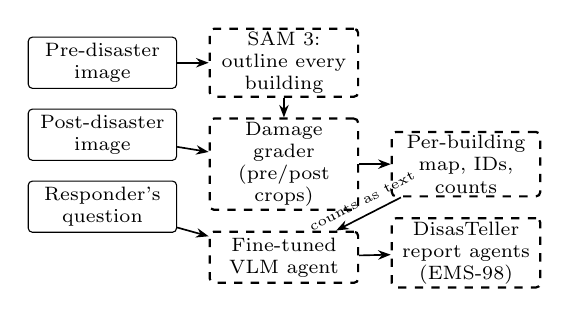
\begin{tikzpicture}[
  node distance=2.5mm and 4mm,
  box/.style={draw, rounded corners=1.5pt, align=center, font=\scriptsize, text width=18mm, minimum height=6.5mm, inner sep=1.2pt},
  fut/.style={box, dashed, thick},
  arr/.style={-{Stealth[length=1.6mm]}, semithick}]
\node[box] (pre) {Pre-disaster image};
\node[fut, right=of pre] (sam) {SAM~3: outline every building};
\node[box, below=of pre] (post) {Post-disaster image};
\node[fut, below=of sam] (grade) {Damage grader (pre/post crops)};
\node[fut, right=of grade] (map) {Per-building map, IDs, counts};
\node[box, below=of post] (q) {Responder's question};
\node[fut, below=of grade] (vlm) {Fine-tuned VLM agent};
\node[fut, below=of map] (rep) {DisasTeller report agents (EMS-98)};
\draw[arr] (pre) -- (sam);
\draw[arr] (sam) -- (grade);
\draw[arr] (post) -- (grade);
\draw[arr] (grade) -- (map);
\draw[arr] (map) -- node[midway, sloped, above, font=\tiny] {counts as text} (vlm);
\draw[arr] (q) -- (vlm);
\draw[arr] (vlm) -- (rep);
\end{tikzpicture}
\caption{Proposed offline triage architecture. Solid boxes are inputs; dashed boxes are CSE499B work. The VLM reads per-building counts as text and drives DisasTeller's report agents on our own model, giving a damage map with building IDs, counts, a survivability heatmap and a report without any cloud API.}
\label{fig:system}
\end{figure}

\subsection{Future Directions and Proposed Architecture}
Our fine-tuning settings now change results by less than run-to-run noise, so the next gains must come from structural changes (Fig.~\ref{fig:system}). \textit{1) Before/after input:} DisasterM3 pairs each post-disaster image with a pre-disaster one; the top five xView2 solutions~\cite{xview2sol} on xBD~\cite{xbd} all compare the two, while our U-Net sees only the post-disaster image. \textit{2) Find buildings, then grade each one:} SAM~3~\cite{sam3}, prompted with ``building'' on the pre-disaster image, lists every building without training, and a small Siamese classifier grades each one from its pre/post crops, turning rare pixels into rare objects (16,682 destroyed instances in our training split) counted one by one. \textit{3) A VLM that plans rather than guesses:} the fine-tuned VLM receives per-building counts as text, calls tools such as the segmenter and an EMS-98 retriever, and drives DisasTeller's report agents on our own model instead of the Gemini API. This also sidesteps the 512-token image cap (CSE499A deviation D4: the reduced image budget needed to train on a 16\,GB T4). \textit{4) Small enough for the field:} 7B$\rightarrow$3B distillation~\cite{seqkd} (notebooks written), 4-bit quantisation and a distilled SAM~3, with speed, memory and accuracy loss measured. A two-day test first checks that SAM~3 runs on a free T4 and finds buildings on DisasterM3.

\subsection{Evaluation Plan}
Segmentation is scored with the E-protocol: per-class IoU, mIoU, Destroyed recall and F2, which weights recall twice as much as precision because a missed destroyed building costs more than a false alarm. The VLM is scored by exact-match accuracy on the six DisasterM3 multiple-choice tasks against the CSE499A results. The system is checked by an offline end-to-end run on held-out images, and distillation by the 3B student's per-task accuracy relative to the 7B teacher.

\section{Timeline}
\textbf{September (done):} ablation sprint. \textbf{October (in progress):} controlled U-Net re-runs (Section~V), then a two-day SAM~3 test. \textbf{Late October to November:} before/after input, two-stage grading, and the VLM agent with offline DisasTeller reports. \textbf{November to December:} 7B$\rightarrow$3B distillation and an edge benchmark; xBD data only if the Destroyed gate still fails. \textbf{December:} integration, final evaluation and report.

\section{Risks and Mitigations}
Table~\ref{tab:risks} lists the main risks; the first and third have already occurred during the sprint.

\begin{table}[t]
\caption{Risk Register}
\label{tab:risks}
\centering
\footnotesize
\setlength{\tabcolsep}{4pt}
\begin{tabular}{@{}>{\raggedright\arraybackslash}p{3.2cm}>{\raggedright\arraybackslash}p{5.0cm}@{}}
\toprule
Risk & Mitigation\\
\midrule
GPU quota (about 30\,h per account per week; 6--7\,h per U-Net run, about 21\,h for UNet++) & Run R1, R6 and E0 first; spread runs over members' accounts; resume each run from its own checkpoint repository\\
Champion misses Destroyed IoU 0.30 & Phase 2: xBD data mapped to our four classes, or a two-stage building-then-damage model\\
Platform drift (Kaggle moved to Python 3.13) & Pin only API-critical libraries; stop on any install error; smoke-test before long runs\\
VLM out of memory at higher resolution & Unlock resolution at inference only; single-image batches; larger free GPUs (P100, L4)\\
3B student loses accuracy & Report per-task retention; keep the 7B as the server model\\
Hallucinated or unsafe guidance & Decision support only; human review; flag low-confidence answers\\
\bottomrule
\end{tabular}
\end{table}

\section{Ethical Considerations}
The system is decision support only: its outputs require expert review before field use, and the interface will say so. Heatmaps are likelihood estimates, not survivor detections. DisasterM3 is used under its non-commercial licence, no imagery of casualties is used, and geographic and disaster-type gaps will be documented in the model cards.

\section{Deliverables}
A stronger segmentation model with a full results table; SAM~3 building finding with per-building damage grades, if the feasibility test passes; offline DisasTeller reports on our fine-tuned VLM, with damage map, counts and survivability heatmap; a distilled Qwen2.5-VL-3B (about 6\,GB) with an edge benchmark; and a final IEEE-format report with code and checkpoints on Hugging Face.

\section{Conclusion}
The CSE499B sprint showed that loss design, not decoder choice, moved the segmentation stage most, lifting mIoU from 0.4619 to 0.5296 and Destroyed IoU from 0.166 to 0.279. The audit then made the numbers trustworthy enough to combine, and the first champion runs reached 0.544 mIoU with TTA under the stricter protocol. The remaining runs aim to close the Destroyed-IoU gap (0.284 against 0.30), and the four future directions turn the resulting segmentation stage into an offline, edge-deployable triage tool for responders.

\newpage
\begin{thebibliography}{00}
\bibitem{disasterm3} J. Wang, W. Xuan, H. Qi, Z. Liu, K. Liu, Y. Wu, H. Chen, J. Song, J. Xia, Z. Zheng, and N. Yokoya, ``DisasterM3: A remote sensing vision-language dataset for disaster damage assessment and response,'' in \textit{Proc. NeurIPS}, 2025, arXiv:2505.21089.
\bibitem{qwen25vl} S. Bai \textit{et al.}, ``Qwen2.5-VL technical report,'' arXiv:2502.13923, 2025.
\bibitem{qlora} T. Dettmers, A. Pagnoni, A. Holtzman, and L. Zettlemoyer, ``QLoRA: Efficient finetuning of quantized LLMs,'' in \textit{Proc. NeurIPS}, 2023.
\bibitem{unet} O. Ronneberger, P. Fischer, and T. Brox, ``U-Net: Convolutional networks for biomedical image segmentation,'' in \textit{Proc. MICCAI}, 2015, pp. 234--241.
\bibitem{crewai} CrewAI, ``CrewAI: A framework for orchestrating role-playing AI agents,'' 2024. [Online]. Available: \url{https://github.com/crewAIInc/crewAI}
\bibitem{disastervqa} A. Al-Mohannadi, A. Firoz, Y. Yang, M. Imran, and F. Ofli, ``DisasterVQA: A visual question answering benchmark dataset for disaster scenes,'' in \textit{Proc. ICWSM}, 2026, arXiv:2601.13839.
\bibitem{vrt} J. Liang \textit{et al.}, ``VRT: A video restoration transformer,'' arXiv:2201.12288, 2022.
\bibitem{xbd} R. Gupta \textit{et al.}, ``Creating xBD: A dataset for assessing building damage from satellite imagery,'' in \textit{Proc. IEEE/CVF CVPR Workshops}, 2019.
\bibitem{focaltversky} N. Abraham and N. M. Khan, ``A novel focal Tversky loss function with improved attention U-Net for lesion segmentation,'' in \textit{Proc. IEEE ISBI}, 2019, pp. 683--687.
\bibitem{lovasz} M. Berman, A. Rannen Triki, and M. B. Blaschko, ``The Lov\'asz-Softmax loss: A tractable surrogate for the optimization of the intersection-over-union measure in neural networks,'' in \textit{Proc. IEEE/CVF CVPR}, 2018, pp. 4413--4421.
\bibitem{copypaste} G. Ghiasi \textit{et al.}, ``Simple copy-paste is a strong data augmentation method for instance segmentation,'' in \textit{Proc. IEEE/CVF CVPR}, 2021, pp. 2918--2928.
\bibitem{unetpp} Z. Zhou, M. M. Rahman Siddiquee, N. Tajbakhsh, and J. Liang, ``UNet++: A nested U-Net architecture for medical image segmentation,'' in \textit{Proc. DLMIA Workshop, MICCAI}, 2018, pp. 3--11.
\bibitem{deeplab} L.-C. Chen, Y. Zhu, G. Papandreou, F. Schroff, and H. Adam, ``Encoder-decoder with atrous separable convolution for semantic image segmentation,'' in \textit{Proc. ECCV}, 2018, pp. 801--818.
\bibitem{seqkd} Y. Kim and A. M. Rush, ``Sequence-level knowledge distillation,'' in \textit{Proc. EMNLP}, 2016, pp. 1317--1327.
\bibitem{sam3} N. Carion \textit{et al.}, ``SAM 3: Segment anything with concepts,'' arXiv:2511.16719, 2025.
\bibitem{xview2sol} Defense Innovation Unit, ``xView2 challenge: Top-five winning solutions,'' 2020. [Online]. Available: \url{https://github.com/DIUx-xView}
\bibitem{resnet} K. He, X. Zhang, S. Ren, and J. Sun, ``Deep residual learning for image recognition,'' in \textit{Proc. IEEE CVPR}, 2016, pp. 770--778.
\end{thebibliography}

\end{document}
